\begin{enumerate}

\item Let us label the output of the LFSR $110100100001010$ as

\[s_0 || s_1 || s_2 || ... || s_{14} \]

where $s_i$ is the $i$th bit of the sequence of bits generated by our LFSR. Then

\begin{align*}
\begin{pmatrix}
s_5 \\ s_6 \\ s_7 \\ s_8 \\ s_9 
\end{pmatrix}
&= 
\begin{pmatrix}
s_0 & s_1 & s_2 & s_3 & s_4 \\
s_1 & s_2 & s_3 & s_4 & s_5 \\
s_2 & s_3 & s_4 & s_5 & s_6 \\
s_3 & s_4 & s_5 & s_6 & s_7 \\
s_4 & s_5 & s_6 & s_7 & s_8 \\
\end{pmatrix} 
\begin{pmatrix}
c_0 \\ c_1 \\ c_2 \\ c_3 \\ c_4
\end{pmatrix} 
\end{align*}

where $c_i$ is the $i$th connection coefficient. Substituting in our values and
solving for the $c_i$s, we have that

\begin{align*}
\Rightarrow 
\begin{pmatrix}
c_0 \\ c_1 \\ c_2 \\ c_3 \\ c_4
\end{pmatrix}
&=
\begin{pmatrix}
1 & 1 & 0 & 1 & 0 \\
1 & 0 & 1 & 0 & 0 \\
0 & 1 & 0 & 0 & 1 \\
1 & 0 & 0 & 1 & 0 \\
0 & 0 & 1 & 0 & 0 
\end{pmatrix}^{-1}
\begin{pmatrix} 0 \\  1 \\ 0 \\ 0 \\ 0 \end{pmatrix} \\
&=
\begin{pmatrix}
0 & 1 & 0 & 0 & 1 \\
1 & 0 & 0 & 1 & 0 \\
0 & 0 & 0 & 0 & 1 \\
0 & 1 & 0 & 1 & 1 \\
1 & 0 & 1 & 1 & 0
\end{pmatrix}
\begin{pmatrix} 0 \\  1 \\ 0 \\ 0 \\ 0 \end{pmatrix} \\
&=
\begin{pmatrix} 1 \\  0 \\ 0 \\ 1 \\ 0 \end{pmatrix}
\end{align*}.

This means that $c_0, c_3$ are 1 with $c_1, c_2, c_4$ being 0.

\begin{figure}[H]
\centering
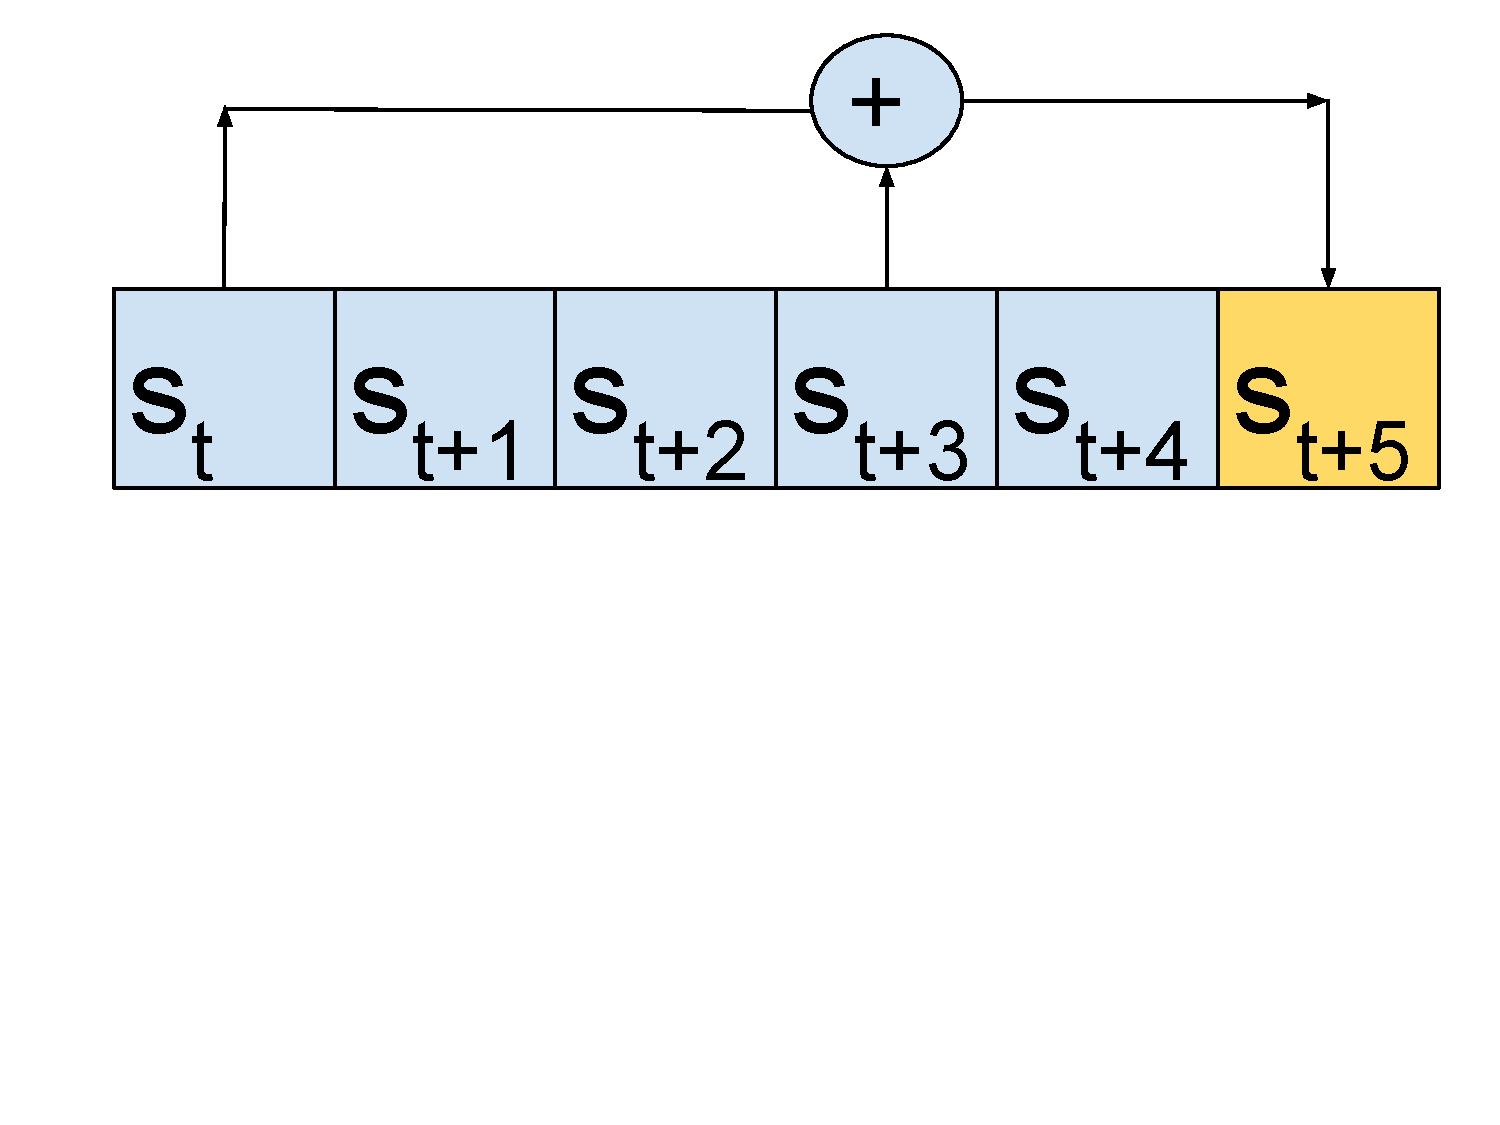
\includegraphics[width=\textwidth]{lfsr.pdf}
\label{fig:lfsr}
\caption{The LFSR for Question 1. Here we depict each bit of the LFSR as a
square, with the current state bits being highlighted in blue. The first and
fourth bits of the LFSR state being XORed to create the new state bit $s_{t+5}$
which will be the fifth bit of the LFSR state after $s_t$ is outputted.}
\end{figure}
\item See Figure \ref{fig:lfsr}. 

\item One characteristic polynomial would be $F(X) = X^5 + X^3 + 1$.

\item If the first $L$ states $S_i$ of an LFSR of length $L$ are linearly
dependent, then there exists $a_0, \dots, a_{L-1} \in \{0, 1\}$ not all $0$
such that \[a_0 S_0 + a_1 S_1 + \dots + a_{L-2} S_{L-2} + a_{L-1} S_{L-1} = 0\].
Let $j$ be the largest integer such that $0 \leq j \leq L-1$ and $a_j \neq 0$. Then
\[a_0 S_0 + a_1 S_1 + \dots + a_{j-1} S_{j-1} = a_j S_j\].  This defines a LFSR
of length $j < L$ with the $i$th connection coefficient defined as \[c_i =
\sum_0^i a_i\] which produces the same sequence as the LFSR of length $L$. 

Therefore, if $L$ is the length of the shortest LFSR tht can produce a
particular sequence, then its first $L$ states have to be linearly independent.
If they're linearly dependent, then there exists a sequence of length $j < L$
which can produce that sequence. 

\end{enumerate}
